%FOR PDFLATEX USE ONLY
\documentclass[a4paper,12pt]{article}

\usepackage{amssymb,amsmath} %math symbols

\usepackage[margin=2cm]{geometry} %paper geometry

\usepackage[utf8]{inputenc} %allows unicode (including russian) source file
\usepackage[russian]{babel} %docment in russian-style
\usepackage[utf8]{inputenc}
%\usepackage[unicode]{hyperref} %links inside of the text
\usepackage[pdftex]{graphicx} %includegraphics pictures
\usepackage{cmlgc} %bold text

\usepackage{array} %arrays

%\usepackage{wrapfig}
%\usepackage{array}
%\usepackage{lipsum}
%\usepackage{esvect}
%\usepackage{hyperref}

\usepackage{subfig}
%\usepackage{calc}
%\usepackage{pgfplots,tikz,circuitikz}
%\usepackage{tkz-euclide}

\begin{document}

\begin{center}
  \LARGE{Работа 4.3.2}\\[0.2cm]
  \LARGE{Дифракция света на ультразвуковой волне в жидкости}\\[0.2cm]
  \large{Стрижак Даниил}\\[0.2cm]
\end{center}  
  

\section{Аннотация}

В работе изучается дифракция света на синусоидальной акустической решетке и наблюдается фазовая решетка методом темного поля.
	
С помощью оптической скамьи, осветителя, двух длиннофокусных объективов, кюветы с жидкостью, кварцевого излучателя с микрометрическим винтом, генератора звуковой частоты, линзы, вертикальной нити на рейтере и микроскопа.


\section{Теоретические сведения}

	В работе используются оптическая скамья, осветитель, два длиннофокусных объектива, кювета с жидкостью, кварцевый излучатель с микрометрическим винтом, генератор звуковой частоты, линза, горизонтальная нить на рейтере, микроскоп. 
	
	При прохождении ультразвуковой волны через жидкость в ней возникают периодические неоднородности коэффициента преломления, создается фазовая решетка, которую мы считаем неподвижной ввиду малости скорости звука относительно скорости света. Показатель
	преломления n изменяется по закону:
	
	\begin{equation}\label{}
	n = n_0 (1 + m \cos \Omega x)
	\end{equation}
	
	Здесь $ \Omega = 2 \pi / \Lambda $ --- волновое число для ультразвуковой волны, $ m $ --- глубина модуляции $ n $ $ (m \ll 1 $).
	
	Положим фазу $ \phi $ колебаний световой волны на передней стенке кюветы равной нулю, тогда на задней поверхности она равна:
	
	\begin{equation}\label{}
	\phi  = k n L = \phi_0 (1 + m \cos \Omega x)
	\end{equation}
	
	Здесь $ L $ --- толщина жидкости в кювете, $ k = 2 \pi / \lambda $ --- волновое число для света.
	
	После прохождения через кювету световое поле есть совокупность плоских волн, распространяющихся под углами $ \theta $, соответствующими максимумам в дифракции Фраунгофера:
	
\begin{minipage}{0.47\textwidth}
\begin{equation}\label{}	
	\Lambda \sin \theta_m = m \lambda
\end{equation}

Этот эффект проиллюстрирован на рисунке 1.

	Зная положение дифракционных максимумов, по формуле (1) легко определить длину ультразвуковой волны, учитывая малость $ \theta $: $ \sin \theta \approx \theta \approx l_m /F  $, где $ l_m $ --- расстояние от нулевого до последнего видимого максимума, $ F $ --- фокусное расстояние линзы. Тогда получим:
	
	\begin{equation}\label{}
	 \Lambda = m \lambda F/ l_m 
	\end{equation}
	Скорость ультразвуковых волн в жидкости, где $ \nu $ --- частота колебаний излучателя:
	
\begin{equation}\label{}
	v = \Lambda \nu 
\end{equation}


\end{minipage}	
\begin{minipage}{0.47\textwidth}
		\begin{center}
		
		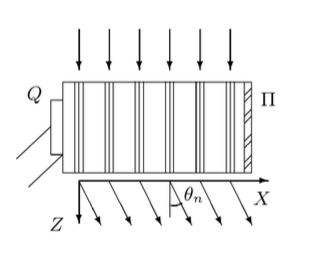
\includegraphics[width=0.9\textwidth]{1.png}
		
		рис. 1. Дифракция световых волн на акустической решетке}
		\label{diff}
		
		\end{center}

\end{minipage}	

\section{Результаты измерений и обработка данных}

\subsection{Определение скорости ультразвука по дифракционной картине}

Схема установки приведена на рисунке 2. Источник света Л через светофильтр Ф и конденсор К освещает вертикальную щель $ S $, находящуюся в фокусе объектива $ O_1 $. После объектива параллельный световой пучок проходит через кювету С перпендикулярно акустической решетке, и дифракционная картина собирается в фокальной плоскости объектива $ O_2 $ , наблюдается при помощи микроскопа М.

Предварительную настройку установки произведем в соответствии с инструкцией с зеленым фильтром, далее в работе используется красный.

\begin{center}
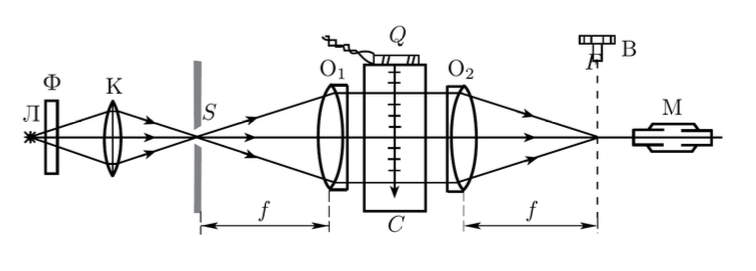
\includegraphics[width=0.7\textwidth]{2.png}

рис. 2. Схема для наблюдения дифракции на акустической решетке
\label{shema1}
\end{center}

Параметры установки: фокусное расстояние объектива $  O_2  $ $ F = 30 $ см, одно деление винта микроскопа составляет 4 мкм, погрешность измерений примем равной  $ \sigma = $ 2 деления, или 8 мкм.

Исследуем изменения дифракционной картины на зеленом свете. При увеличении частоты УЗ-генератора и приближении к 1,17 МГц проявляется дифракционная решетка: расстояние между максимумами растет.

Измерим положения $ x_m $ дифракционных максимумов с помощью микроскопического винта для четырех частот. Результаты измерений занесены в таблицы 1-4 ниже. На основе каждой таблицы построены графики зависимости $ x_m (m) $, они изображены на рисунках 3-6. Коэффициенты углов наклонов прямых для всех зависимостей сведены в таблицу 5. 

\

\newline

\begin{minipage}{0.47\textwidth}
\begin{center}
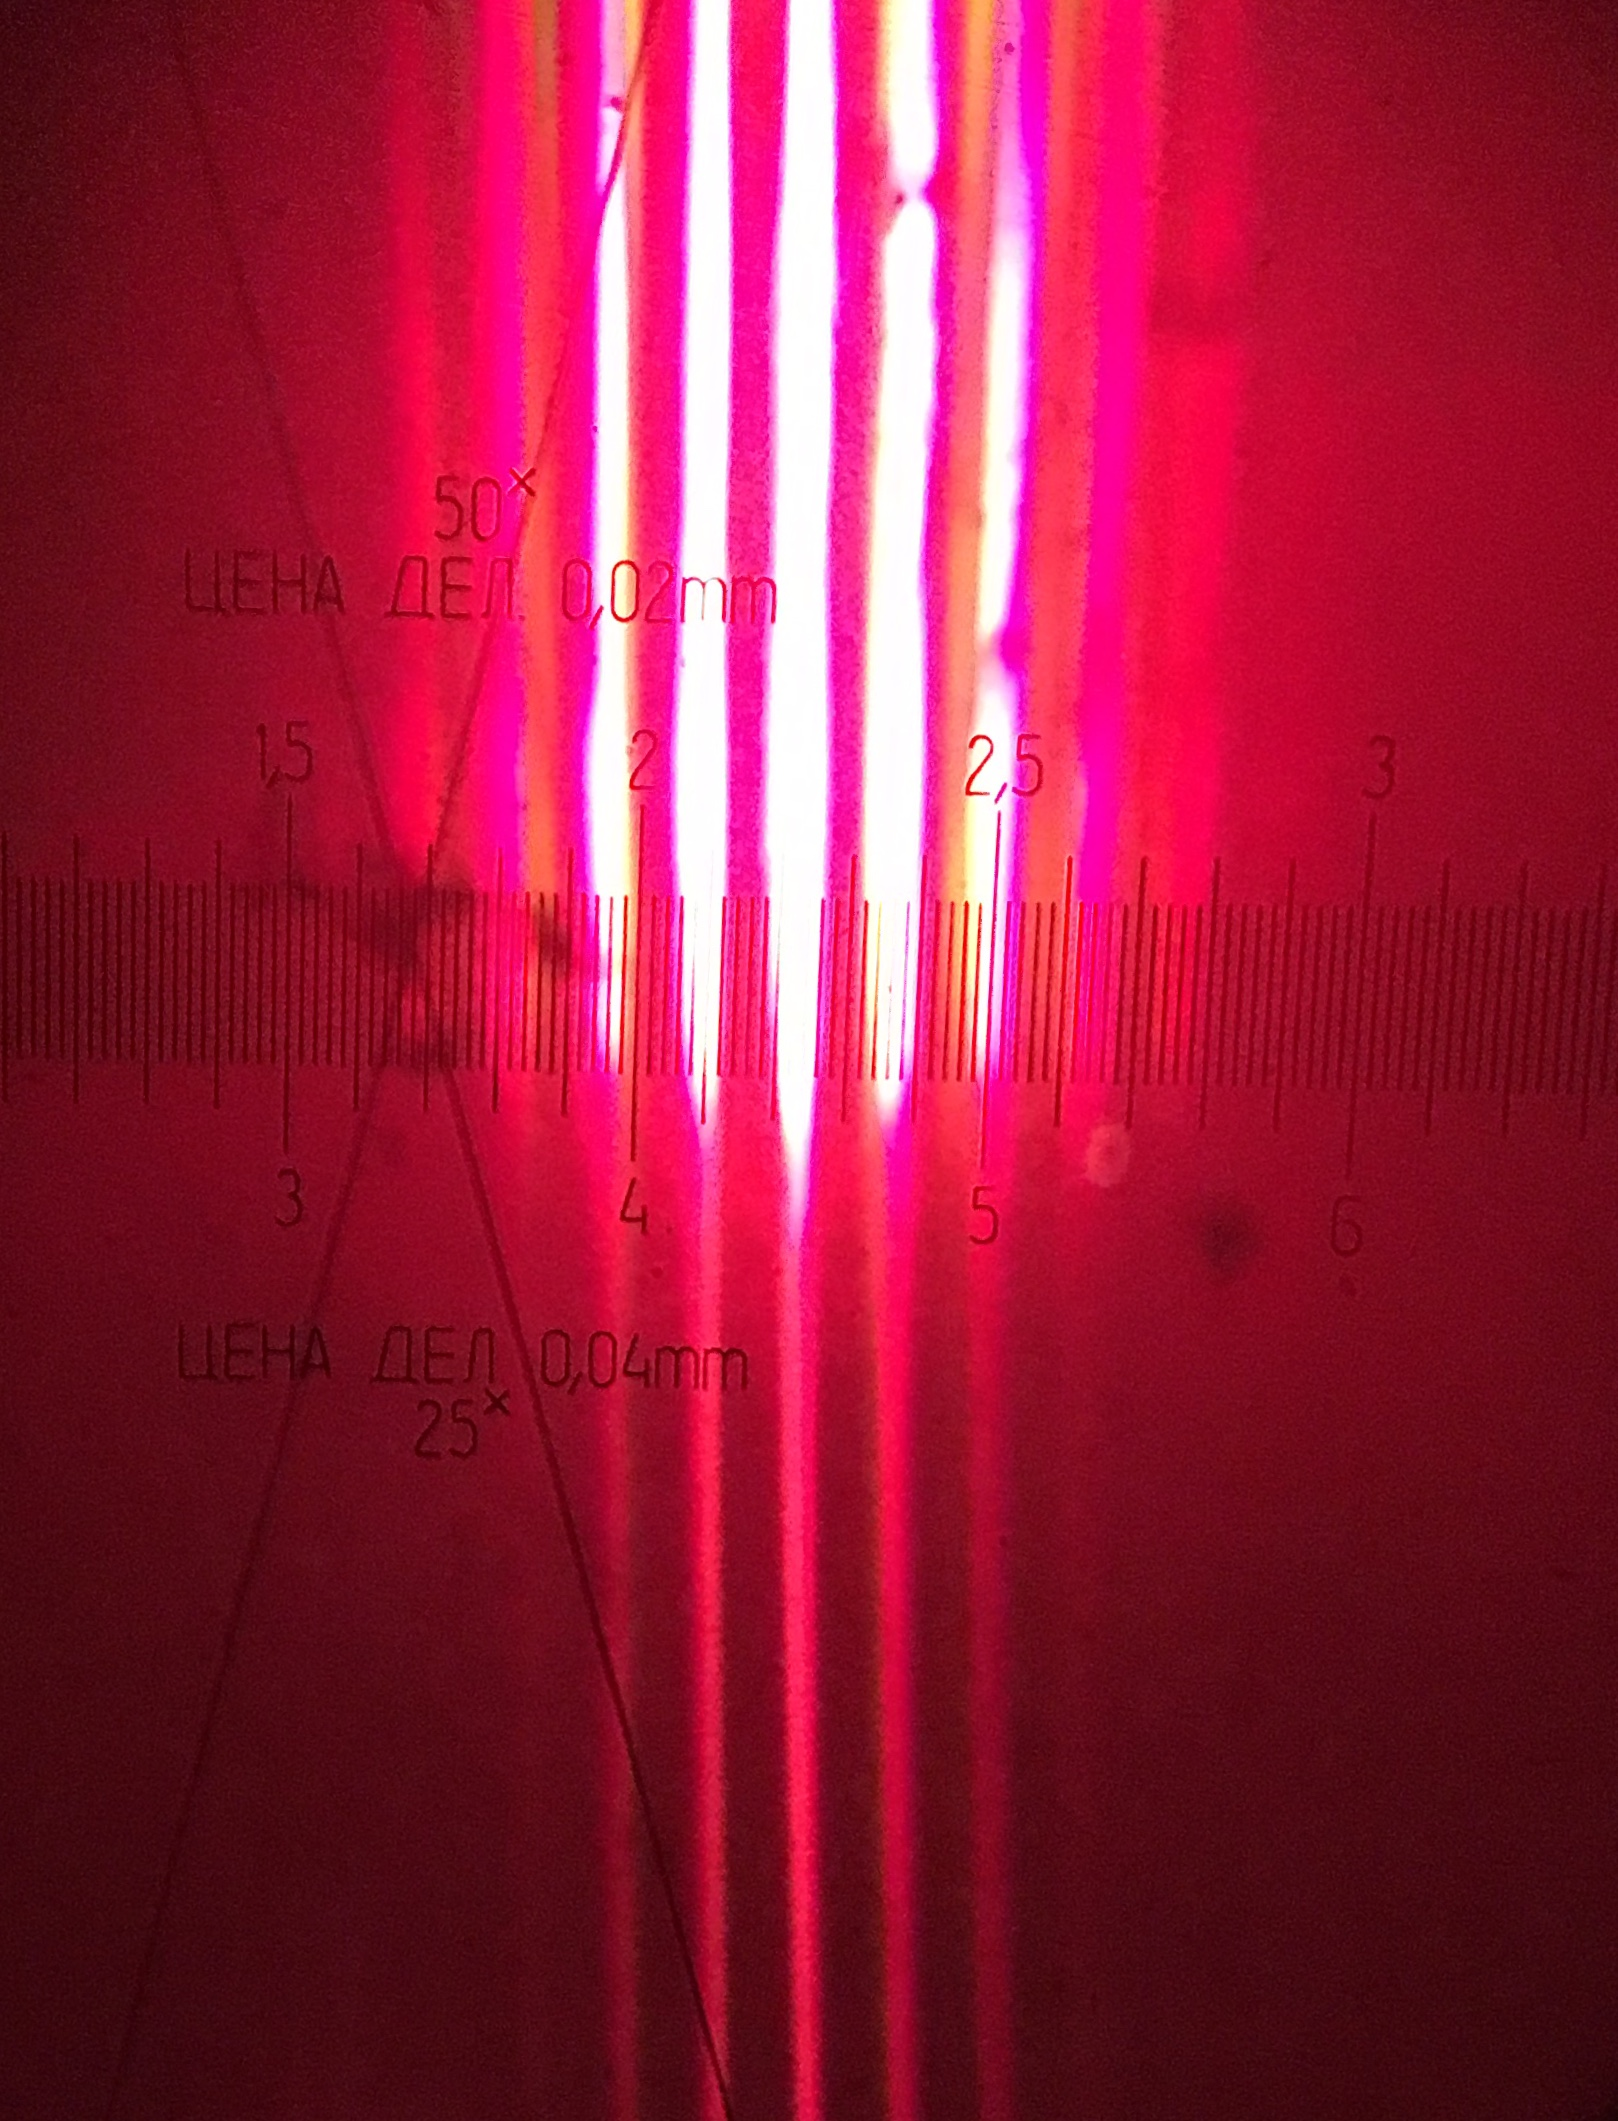
\includegraphics[width=0.7\textwidth]{a.jpg}

Полученная картина
\end{center}
\end{minipage}	
\begin{minipage}{0.47\textwidth}
\begin{center}
\begin{center}
		\begin{tikzpicture}[scale = 1.0]
		\begin{axis}[
		axis lines = left,
		ylabel = {$x_m, \ мкм$},
		xlabel = {$m$},
		minor grid style={black, line width=0.05pt},
		major grid style={solid,black, line width=0.3pt},
		xmin=-5, xmax=5,
		ymin=0, ymax=3500,
		ymajorgrids = true,
		xmajorgrids = true,
		yminorgrids = true,
		xminorgrids = true,
		minor tick num = 4
		]
		\addplot+[only marks ] plot[error bars/.cd, y dir=both, y explicit]
		coordinates {
			(-4,450)
			(-3,730)
			(-2,1080)
			(-1,1370)
			(0,1730)
			(1,2060)
			(2,2360)
			(3,2700)
			(4,2950)
			
		};
		
		\addplot[blue, domain=-8:8]{330*x+1700};
		\end{axis}

		\end{tikzpicture}
График зависимости $x_m(m)$ при частоте генератора $\nu$ = 1,17 МГц	
\end{center}

\end{center}
\end{minipage}	

\

\newline

\begin{center}
\begin{tabular}{|c|c|c|c|c|c|c|c|c|c|}
\hline
$m$ &-4&-3&-2&-1&0&1&2&3&4\\
\hline
$x_m, \ мкм$ &450&730& 1080&1370&1730&2060&2360&2700&2950\\
\hline
\end{tabular}

\

\newline

Таблица 1. Измерение координаты m-ого максимума $x_m$ дифракционной картины при частоте генератора $\nu$ = 1,17 МГц
\end{center}
	
\

\newline

\begin{minipage}{0.47\textwidth}
\begin{center}
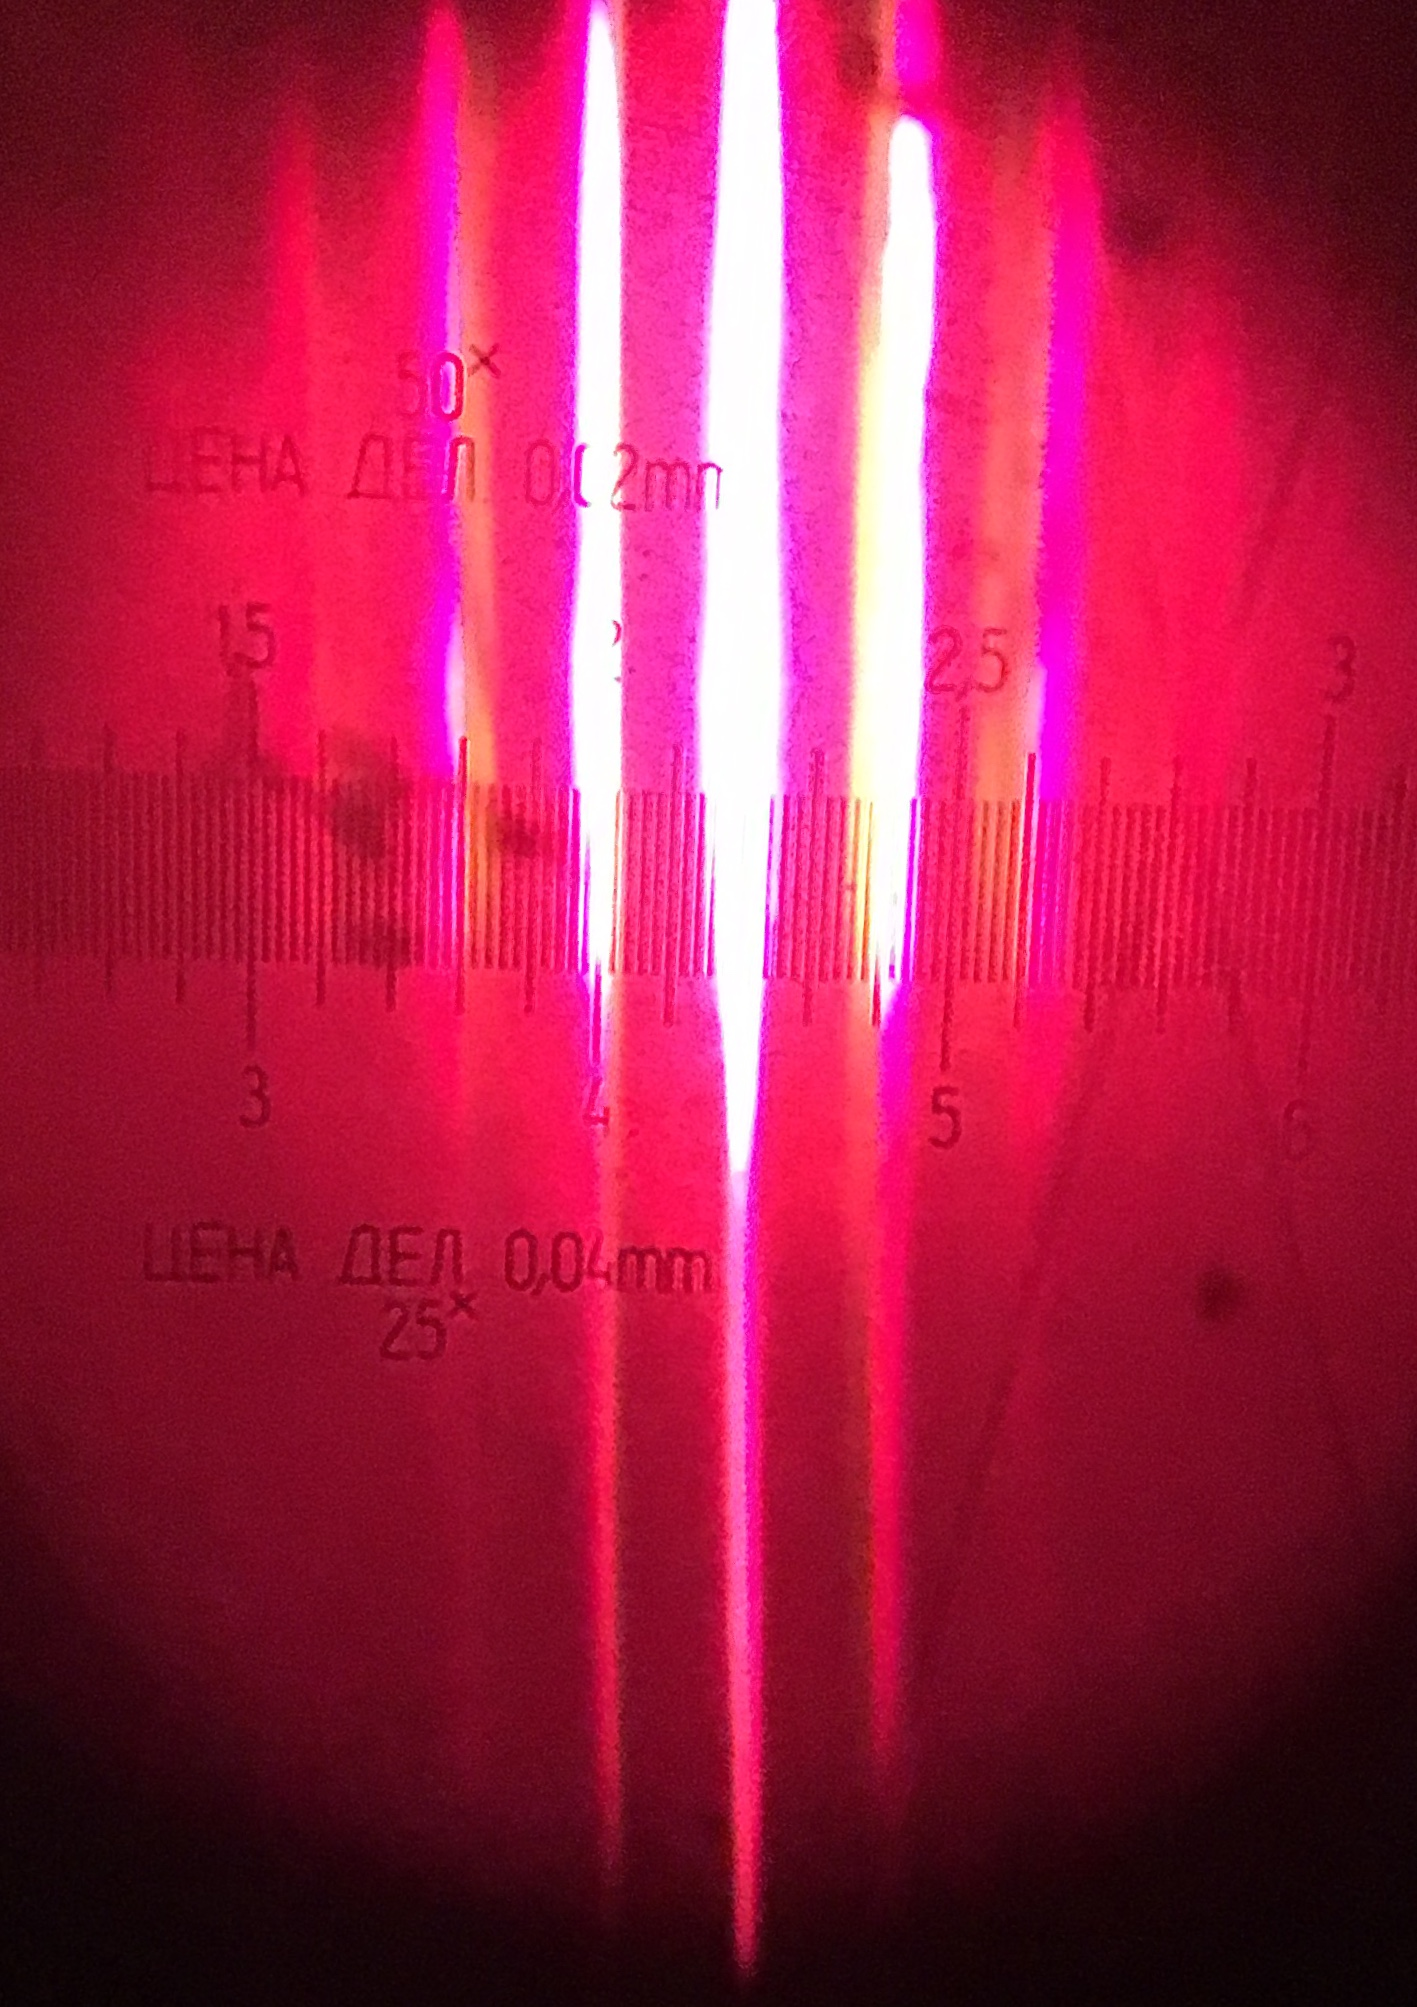
\includegraphics[width=0.7\textwidth]{b.jpg}

Полученная картина
\end{center}
\end{minipage}	
\begin{minipage}{0.47\textwidth}
\begin{center}
\begin{center}
		\begin{tikzpicture}[scale = 1.0]
		\begin{axis}[
		axis lines = left,
		ylabel = {$x_m, \ мкм$},
		xlabel = {$m$},
		minor grid style={black, line width=0.05pt},
		major grid style={solid,black, line width=0.3pt},
		xmin=-4, xmax=4,
		ymin=0, ymax=3500,
		ymajorgrids = true,
		xmajorgrids = true,
		yminorgrids = true,
		xminorgrids = true,
		minor tick num = 4
		]
		\addplot+[only marks ] plot[error bars/.cd, y dir=both, y explicit]
		coordinates {
			
			(-3,50)
			(-2,460)
			(-1,1150)
			(0,1590)
			(1,2110)
			(2,2710)
			(3,3280)
			
			
		};
		
		\addplot[blue, domain=-8:8]{530*x+1650};
		\end{axis}

		\end{tikzpicture}
График зависимости $x_m(m)$ при частоте генератора $\nu$ = 1,82 МГц	
\end{center}

\end{center}
\end{minipage}	

\

\newline

\begin{center}
\begin{tabular}{|c|c|c|c|c|c|c|c|}
\hline
$m$ &-3&-2&-1&0&1&2&3\\
\hline
$x_m, \ мкм$ &50&460& 1150&1590&2110&2710&3280\\
\hline
\end{tabular}

\

\newline

Таблица 2. Измерение координаты m-ого максимума $x_m$ дифракционной картины при частоте генератора $\nu$ = 1,82 МГц
\end{center}	

\newpage

\

\newline

\begin{minipage}{0.47\textwidth}
\begin{center}
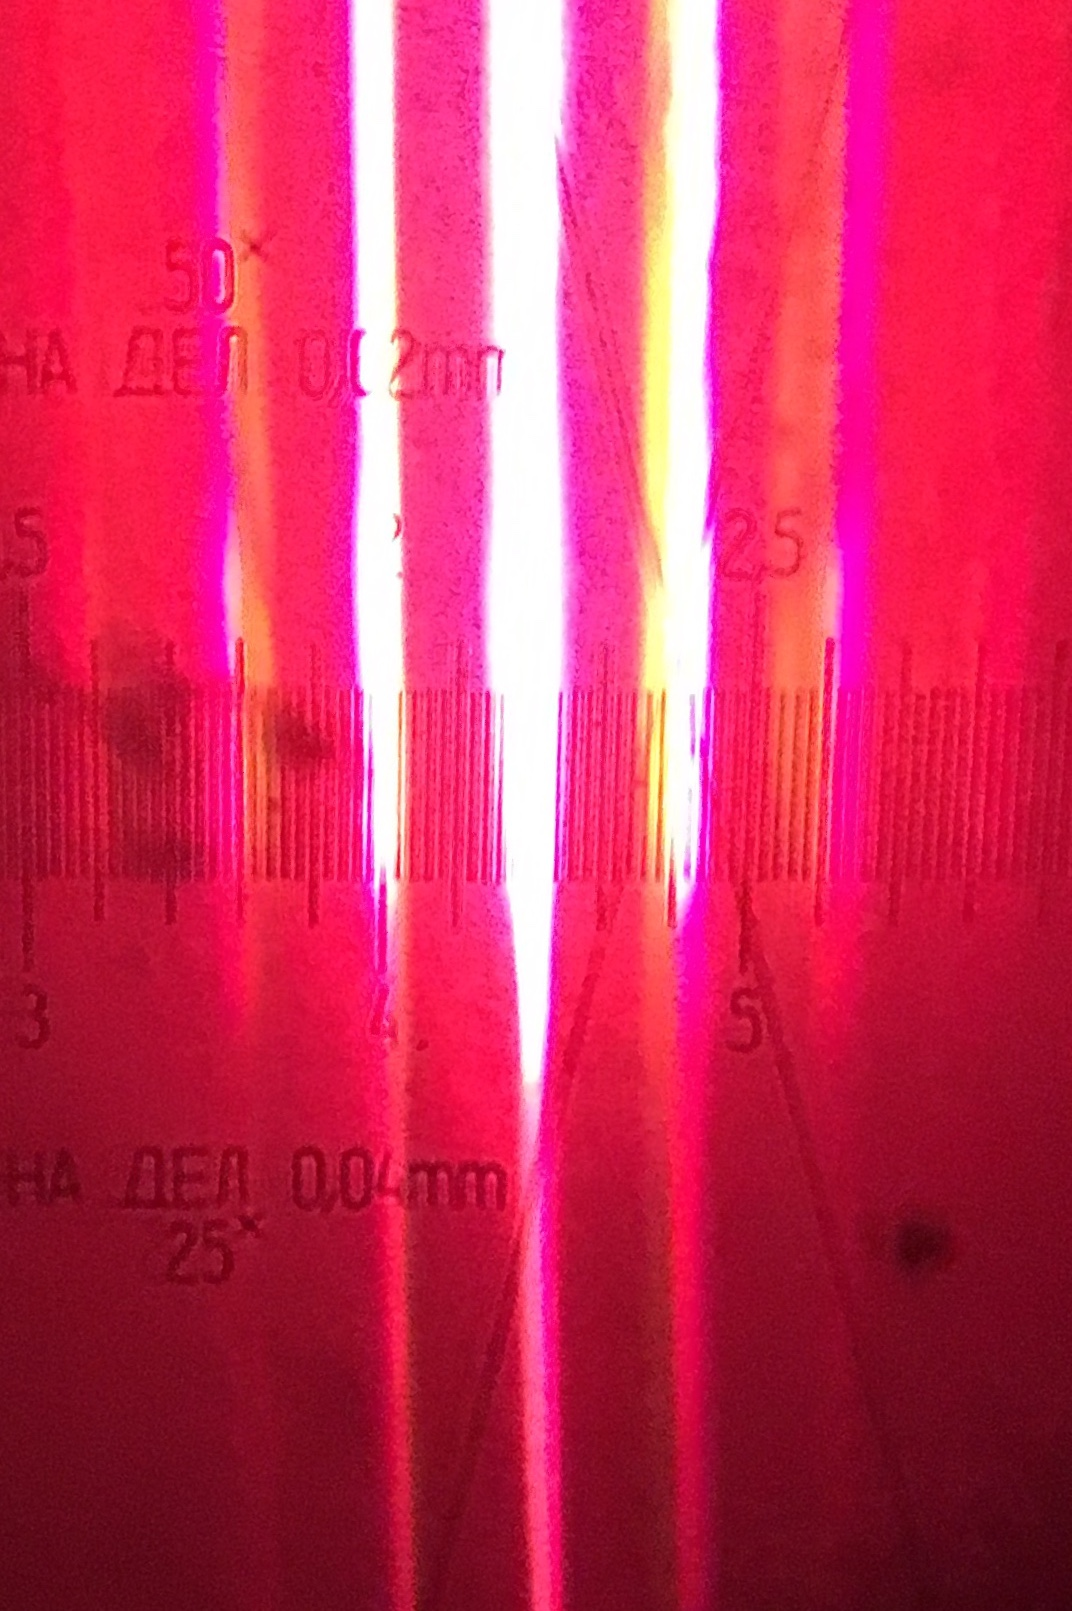
\includegraphics[width=0.7\textwidth]{c.jpg}

Полученная картина
\end{center}
\end{minipage}	
\begin{minipage}{0.47\textwidth}
\begin{center}
\begin{center}
		\begin{tikzpicture}[scale = 1.0]
		\begin{axis}[
		axis lines = left,
		ylabel = {$x_m, \ мкм$},
		xlabel = {$m$},
		minor grid style={black, line width=0.05pt},
		major grid style={solid,black, line width=0.3pt},
		xmin=-4, xmax=4,
		ymin=0, ymax=3500,
		ymajorgrids = true,
		xmajorgrids = true,
		yminorgrids = true,
		xminorgrids = true,
		minor tick num = 4
		]
		\addplot+[only marks ] plot[error bars/.cd, y dir=both, y explicit]
		coordinates {
			
			(-3,460)
			(-2,790)
			(-1,1230)
			(0,1610)
			(1,2030)
			(2,2540)
			(3,3000)
			
			
		};
		
		\addplot[blue, domain=-8:8]{450*x+1650};
		\end{axis}

		\end{tikzpicture}
График зависимости $x_m(m)$ при частоте генератора $\nu$ = 1,55 МГц	
\end{center}

\end{center}
\end{minipage}	

\

\newline

\begin{center}
\begin{tabular}{|c|c|c|c|c|c|c|c|}
\hline
$m$ &-3&-2&-1&0&1&2&3\\
\hline
$x_m, \ мкм$ &460&790& 1230&1610&2030&2540&3000\\
\hline
\end{tabular}

\

\newline

Таблица 3. Измерение координаты m-ого максимума $x_m$ дифракционной картины при частоте генератора $\nu$ = 1,55 МГц
\end{center}

\

\newline

\begin{minipage}{0.47\textwidth}
\begin{center}
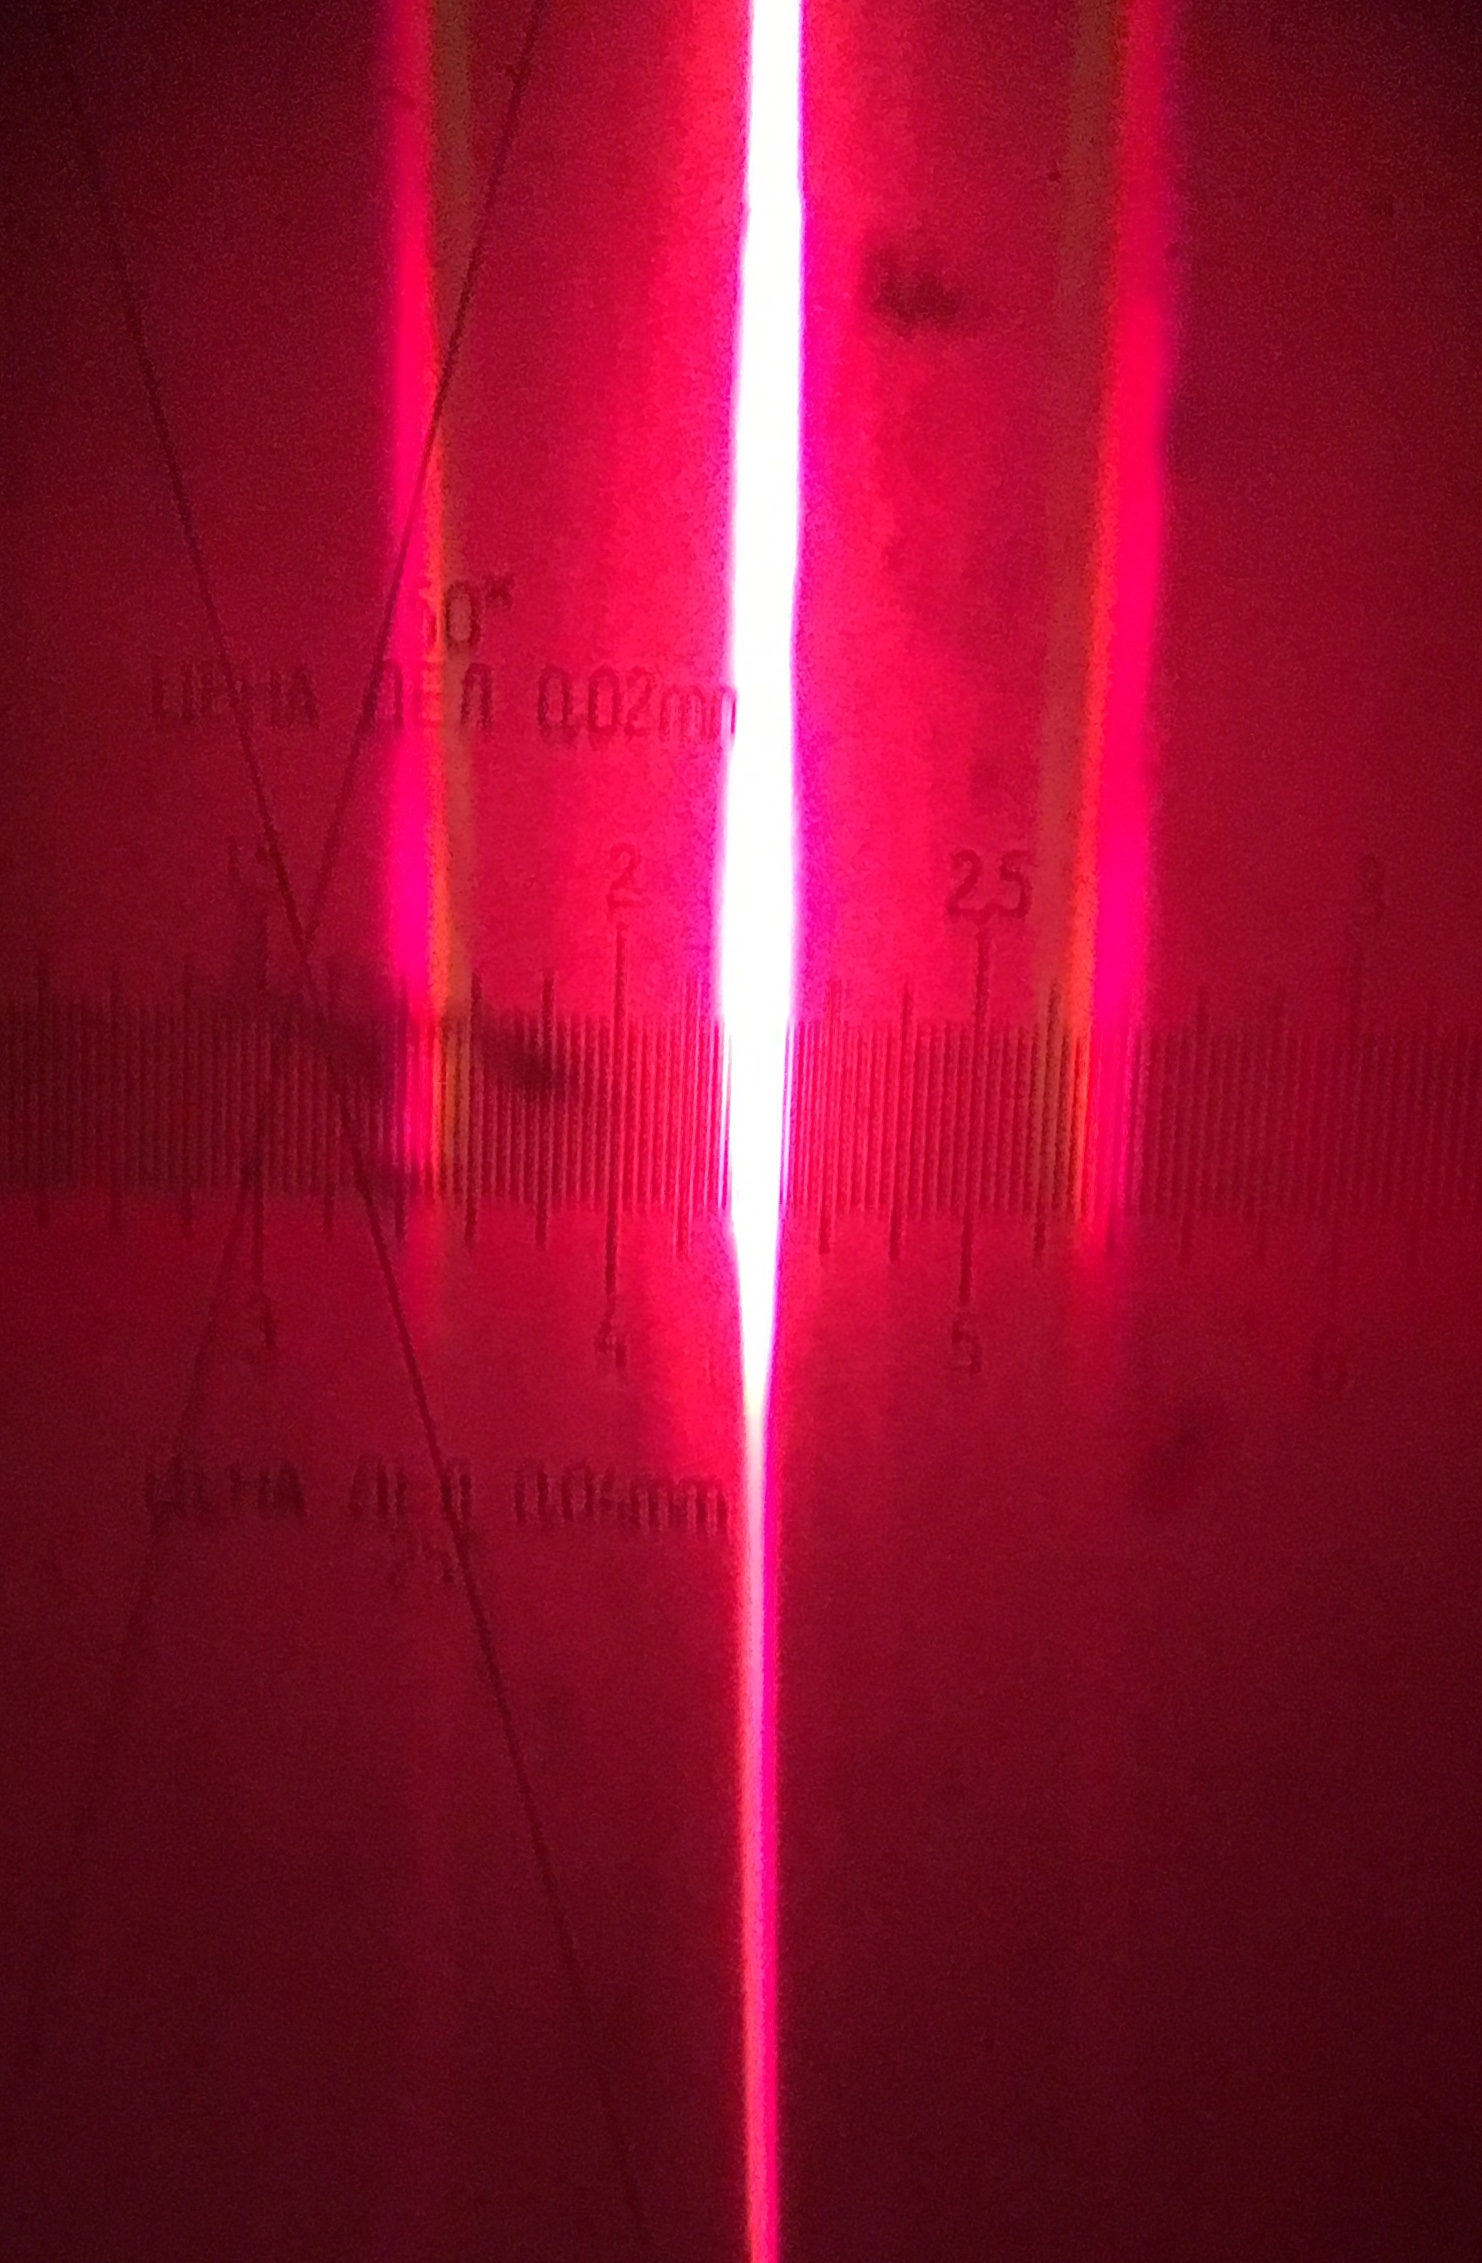
\includegraphics[width=0.7\textwidth]{d.jpg}

Полученная картина
\end{center}
\end{minipage}	
\begin{minipage}{0.47\textwidth}
\begin{center}
\begin{center}
		\begin{tikzpicture}[scale = 1.0]
		\begin{axis}[
		axis lines = left,
		ylabel = {$x_m, \ мкм$},
		xlabel = {$m$},
		minor grid style={black, line width=0.05pt},
		major grid style={solid,black, line width=0.3pt},
		xmin=-3, xmax=3,
		ymin=0, ymax=5500,
		ymajorgrids = true,
		xmajorgrids = true,
		yminorgrids = true,
		xminorgrids = true,
		minor tick num = 3
		]
		\addplot+[only marks ] plot[error bars/.cd, y dir=both, y explicit]
		coordinates {
			
			
			(-2,440)
			(-1,1500)
			(0,2790)
			(1,3730)
			(2,5070)
			
			
			
		};
		
		\addplot[blue, domain=-8:8]{1100*x+2600};
		\end{axis}

		\end{tikzpicture}
График зависимости $x_m(m)$ при частоте генератора $\nu$ = 3.96 МГц	
\end{center}

\end{center}
\end{minipage}	

\

\newline

\begin{center}
\begin{tabular}{|c|c|c|c|c|c|}
\hline
$m$ &-2&-1&0&1&2\\
\hline
$x_m, \ мкм$ &440&1500& 2790&3730&5070\\
\hline
\end{tabular}

\

\newline

Таблица 4. Измерение координаты m-ого максимума $x_m$ дифракционной картины при частоте генератора $\nu$ = 3.96 МГц
\end{center}


\begin{minipage}{0.47\textwidth}
Из зависимости наклона графиков от частоты рассчитаем скорость звука в воде по формулам (2.4) и (2.5). Откуда получаем, что скорость звука равна $$1513 \pm 35\ м/с,$$ что соответствует табличным данным в пределах погрешности измерений и эксперимента -- 1490 м/с. 
\end{minipage}
\begin{minipage}{0.47\textwidth}
\begin{center}
		\begin{tikzpicture}[scale = 1.0]
		\begin{axis}[
		axis lines = left,
		ylabel = {$b,\ мкм$},
		xlabel = {$\nu, \ МГц$},
		minor grid style={black, line width=0.05pt},
		major grid style={solid,black, line width=0.3pt},
		xmin=1, xmax=4.25,
		ymin=200, ymax=1200,
		ymajorgrids = true,
		xmajorgrids = true,
		yminorgrids = true,
		xminorgrids = true,
		minor tick num = 3
		]
		\addplot+[only marks ] plot[error bars/.cd, y dir=both, y explicit]
		coordinates {
			
			
			(1.17,330)
			(1.55,450)
			(1.82,520)
			(3.96,1100)
			
			
			
		};
		
		\addplot[blue, domain=-8:8]{300*x-40};
		\end{axis}

		\end{tikzpicture}
График зависимости $b_m(\nu)$
\end{center}

\end{minipage}

\section{Определение скорости ультразвука методом темного поля}

Для наблюдения акустической решетки используется метод темного поля, который заключается в устранении центрального дифракционного максимума с помощью непрозрачного экрана. Схема установки показана на рисунке.

	\begin{center}

	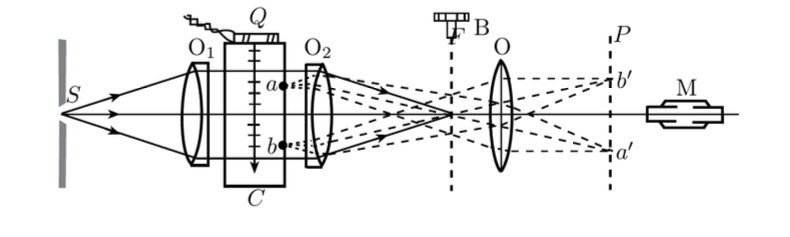
\includegraphics[width=0.7\textwidth]{3.png}
	
	Схема для наблюдения дифракции методом темного поля
	\label{shema2}
\end{center}

Приставим к задней стенке (для светового луча) кюветы стеклянную пластинку с миллиметровыми делениями; сфокусируем микроскоп на изображение пластинки. Определим цену деления окулярной шкалы микроскопа, совместив ее с миллиметровыми делениями: в 1 делении миллиметровой шкалы убирается 1 большое деление окулярной. Значит, цена деления окулярной шкалы: $ C = $ 1 мм.

Без применения метода темного поля звуковая решетка не наблюдается. Закроем нулевой максимум горизонтальной нитью. Таким образом, осевая составляющая фазово-модулированной волны поглощается, а боковые остаются без изменения. Получившееся поле: 

\begin{equation}\label{}
f(x) = \dfrac{im}{2} e^{i\Omega x} +  \dfrac{im}{2} e^{-i\Omega x} = im \cos \Omega x \te I(x) = m^2 \cos ^2 \Omega x = m^2 \dfrac{1 + \cos ^2 2 \Omega x}{2}
\end{equation}

Отсюда получаем, что расстояние между темными полосами есть $ \Lambda/2 $.

\newpage

Проведем измерение длины ультразвуковой волны, приняв ошибку равной цене деления окулярной шкалы. В таблице 6 содержатся количество маленьких делений окулярной шкалы N (цена деления $ C = 1 $), соответствующее $ n $ темным полосам акустической решетки.
Формулы для расчета длины волны ультразвука $ \Lambda $ и скорости распространения $ v $ в воде:
\begin{equation}\label{}
\Lambda/2  = NC/(n - 1),  \qquad v = \nu\Lambda
\end{equation}

Картины наблюдения получились на другой установке, и только при частотах $\nu_1 = 1.22\ МГц$ и $\nu_2 = 2.97 \ МГц$, с помощью этих данных можно определить скорость звука и длину волны. 

В первом случае: $\Lambda = 1.29\pm0.04 \ мм$ и $v = 1570 \pm 60\ м/с$. 

Во втором случае: $\Lambda = 0.53\pm0.04 \ мм$ и $v = 1510 \pm 60\ м/с$

\

\newline


\begin{minipage}{0.47\textwidth}
\begin{center}
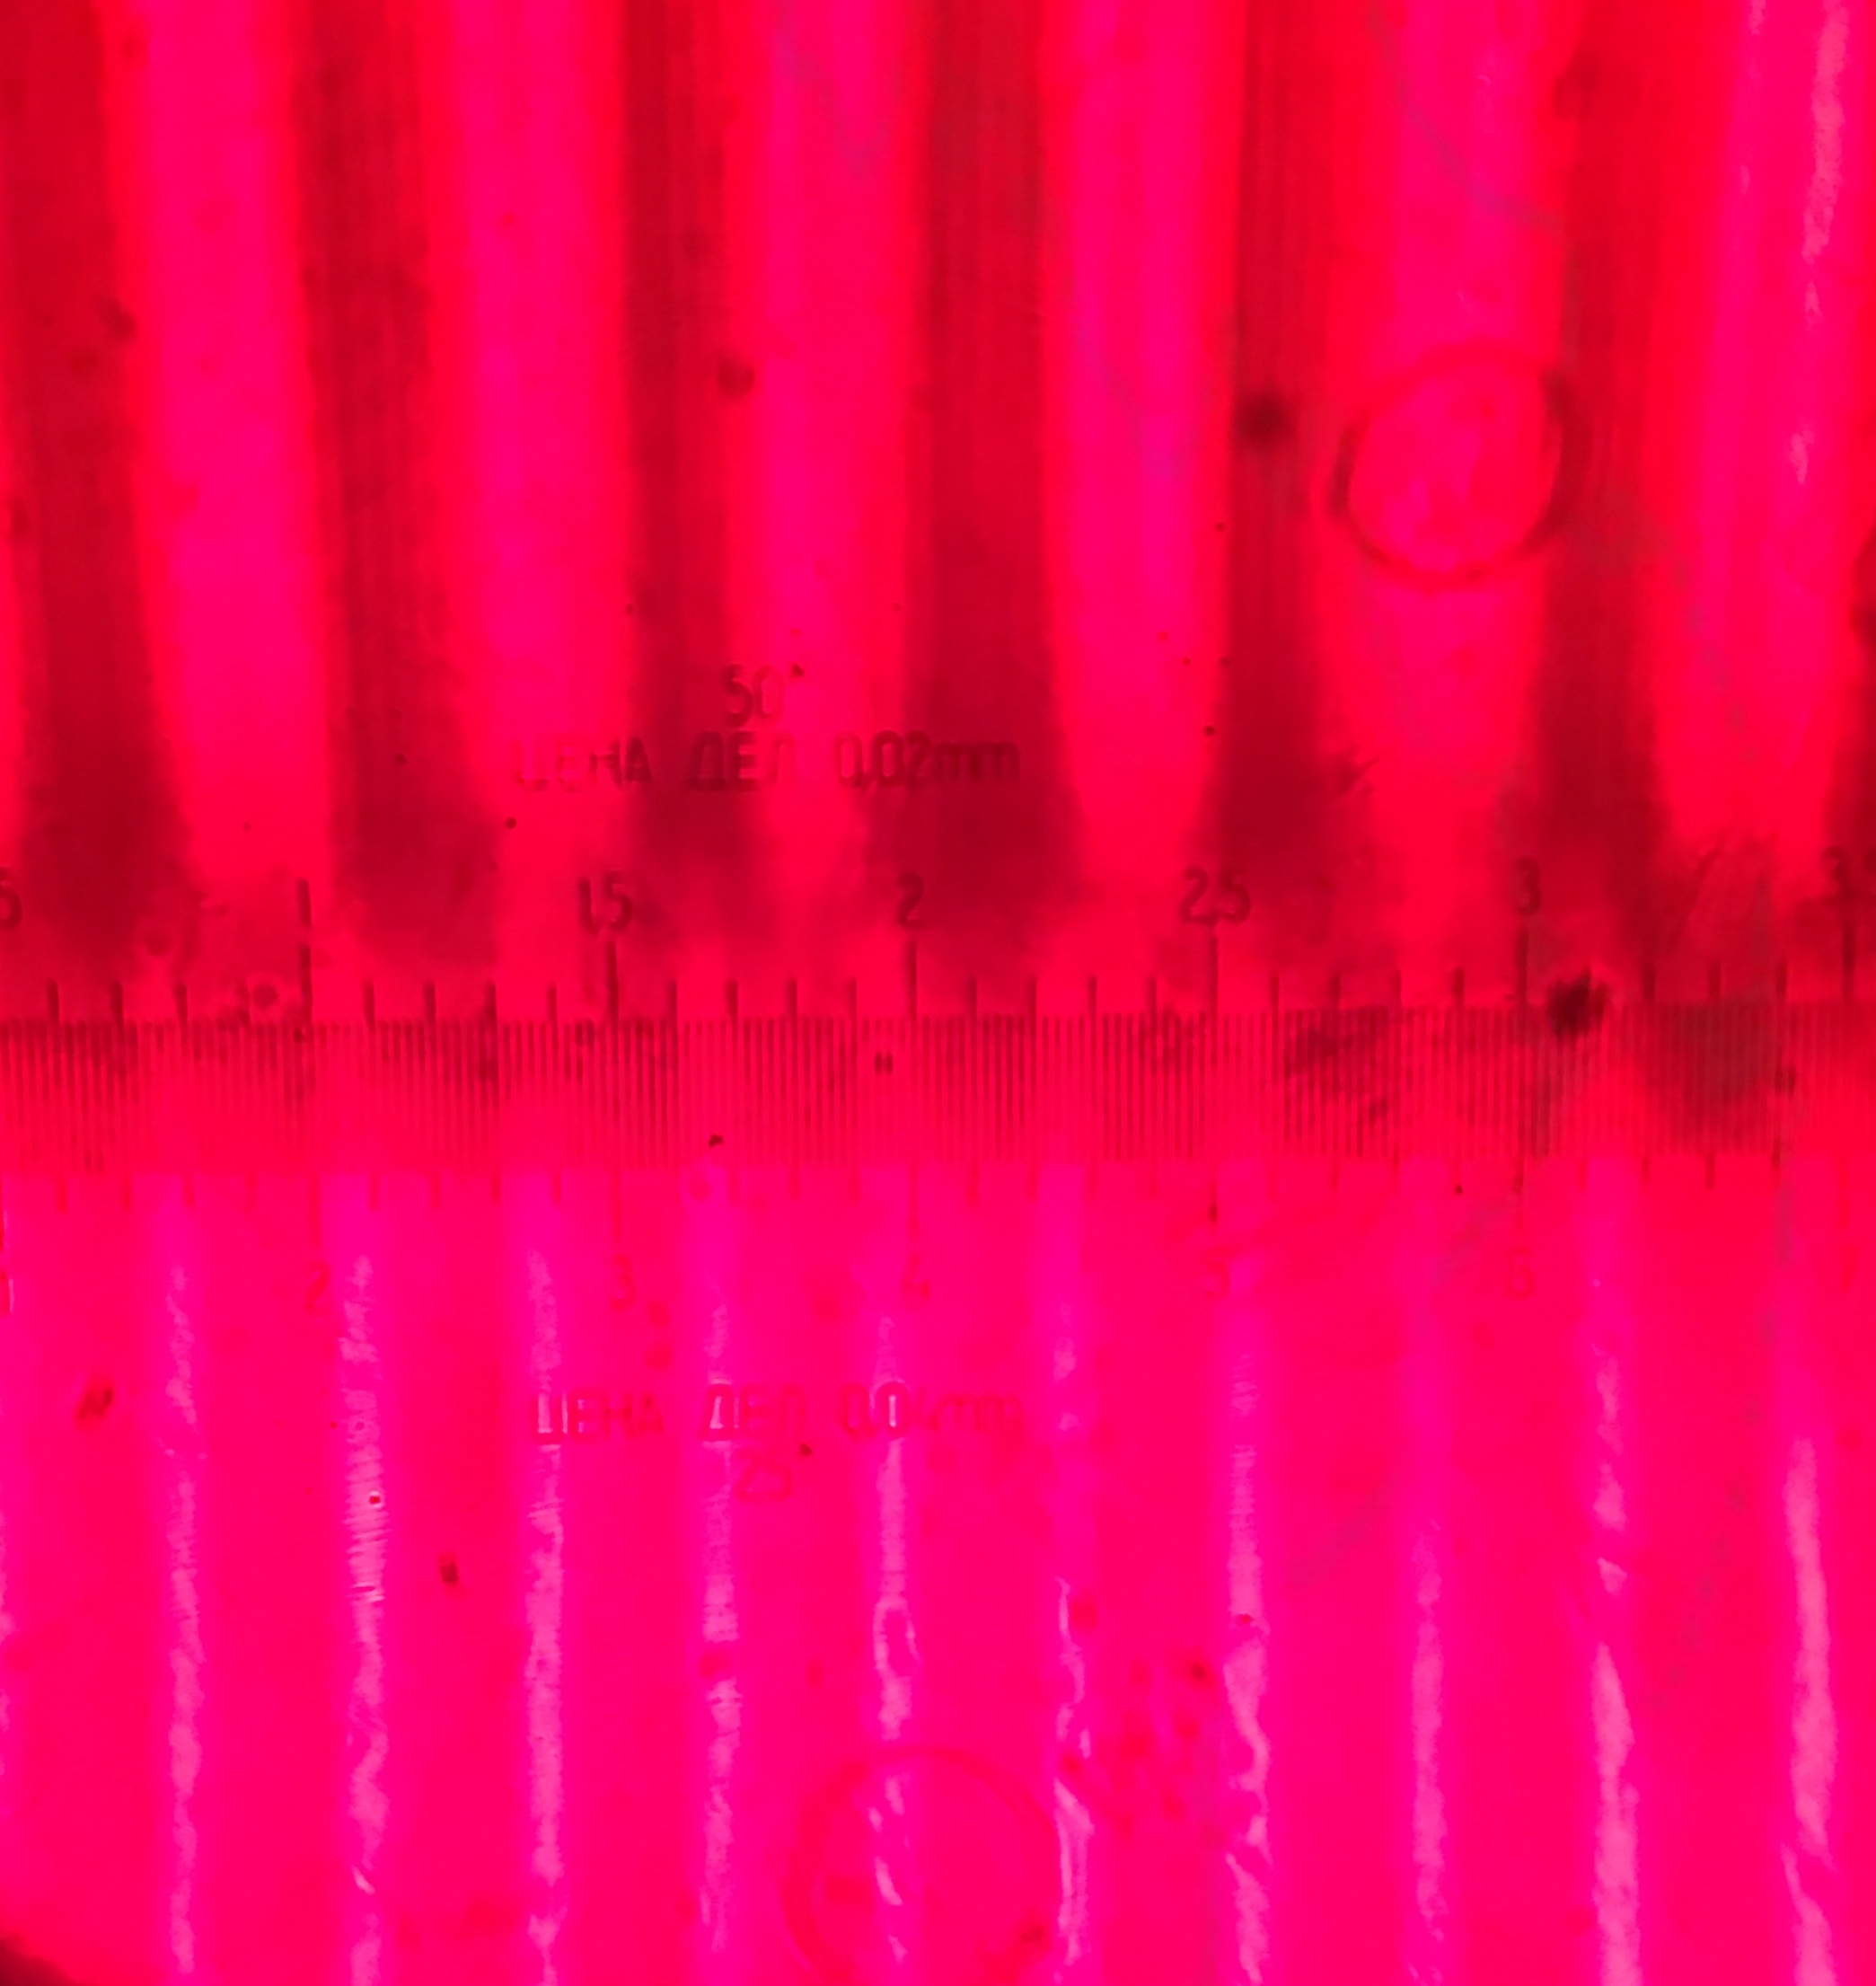
\includegraphics[width=0.7\textwidth]{1.jpg}
	
	Наблюдаемая картина при частоте\\ 1.22 МГц
\end{center}
\end{minipage}
\begin{minipage}{0.47\textwidth}
\begin{center}
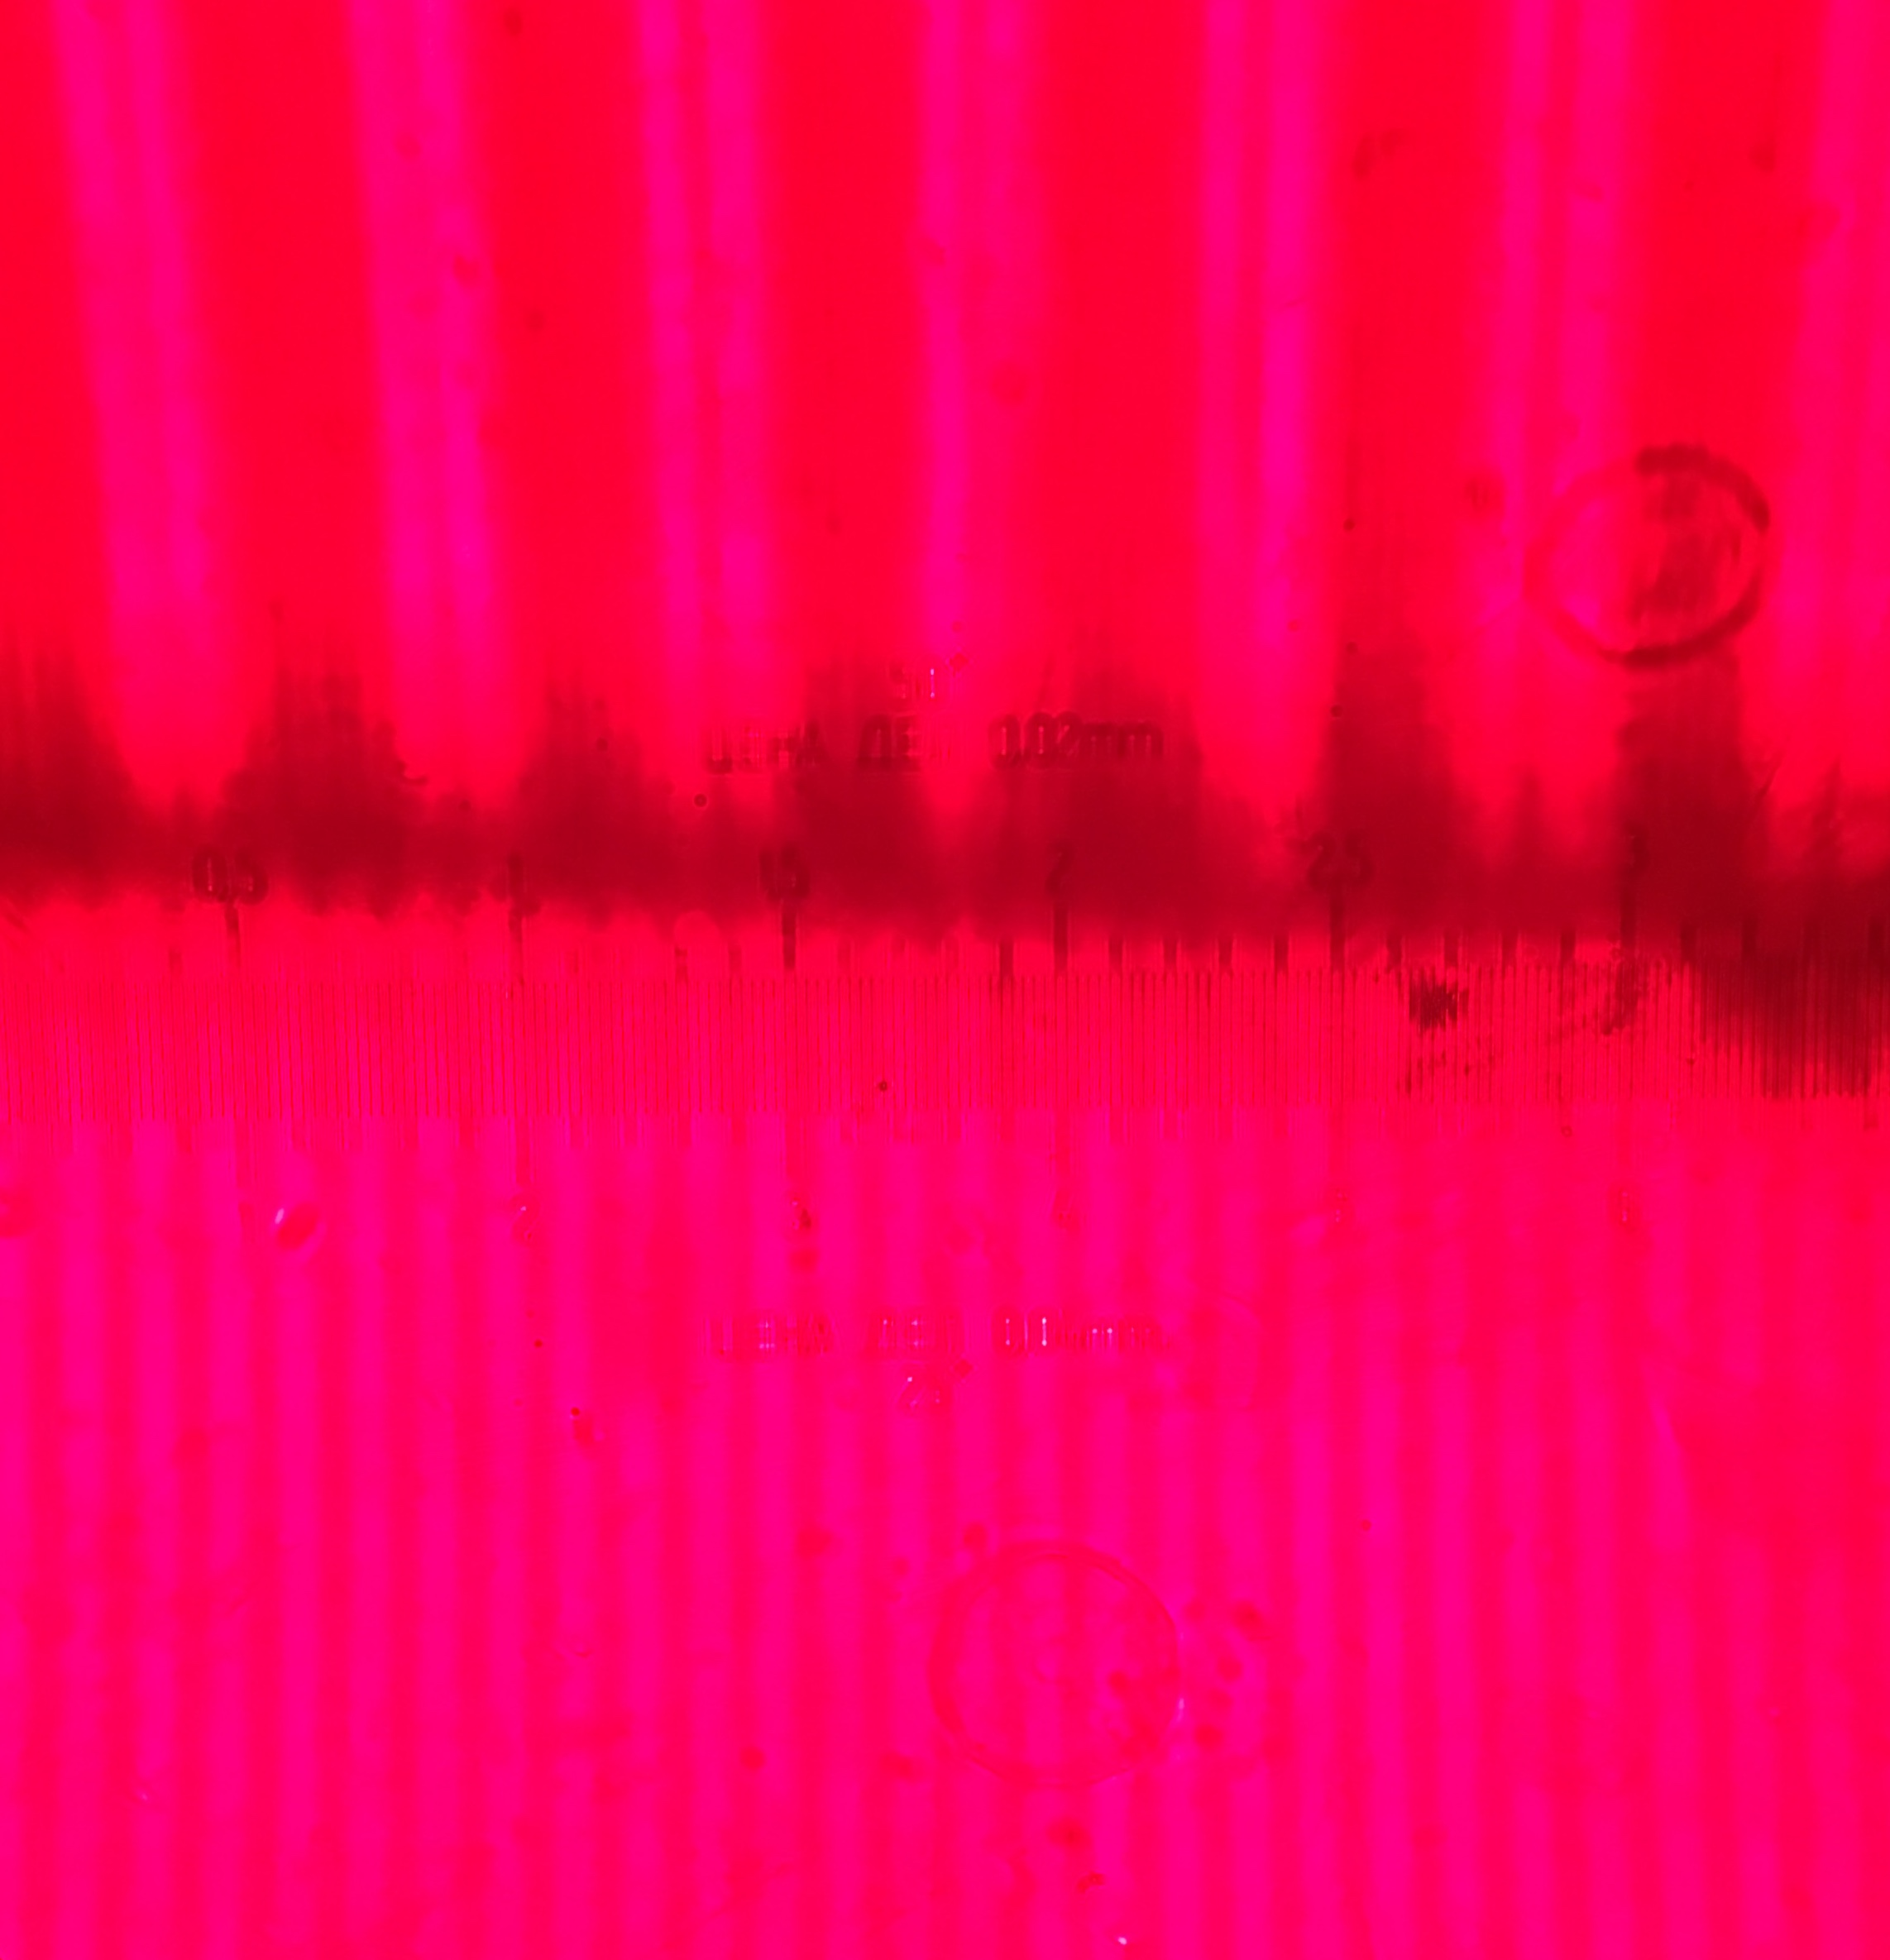
\includegraphics[width=0.7\textwidth]{2.jpg}
	
	Наблюдаемая картина при частоте\\ 2.97 МГц
\end{center}
\end{minipage}

\section{Вывод}

В работе изучена дифракция света на акустической решетки, рассчитаны длина волны ультразвука и скорость его распространения в воде. Решетка наблюдалась методом
темного поля.

Ошибка при определении $ \Lambda $ и $ v $ не превышает 2\%. Согласно справочным данным, при комнатной температуре скорость ультразвуковой волны в воде составляет примерно 1490 м/с. Значения, полученные экспериментально, с достаточной точностью соотносятся с ними.

Ошибка при таком определении скорости звука больше, чем в первой части работы, и
составляет около 5\%. Сами значения тоже получились больше.

\end{document}
